\documentclass[10pt,a4paper]{article}
\usepackage[english]{babel}
\usepackage[utf8]{inputenc}
\usepackage{amsmath}
\usepackage{amsfonts}
\usepackage{amssymb}
\usepackage{graphicx}
\usepackage{float}

%link to documentation: 
%https://ackrep-doc.readthedocs.io/en/latest/devdoc/contributing_data.html

\begin{document}
	\part*{Model Documentation of the \\ Flyback Converter} % MUST - Add Model Name 
	
	%%%%%%%%%%%%%%%%%%%%%% NOMENCLATURE %%%%%%%%%%%%%%%%%%%%%%%%%%%
	
	\section{Nomenclature} % MUST
	\subsection{Nomenclature for Model Equations} % MUST
	
	%variables for model equations
	\begin{tabular}{ll}
		$L$ & inductivity of the inductor \\
		$C$ & capacity of the capacitor \\
		$R$ & resistance of the load \\
		$U_E$ & input voltage \\
		$k$ & transmission ratio of the transformer \\
		$i_L$ & current through the inductor \\
		$u_C$ & voltage over the capatitor \\
		$d$ & duty ratio of the switch \\
			
	\end{tabular}
	 
	\subsection{Circuit Diagram}
	\begin{figure}[H]
		\centering
		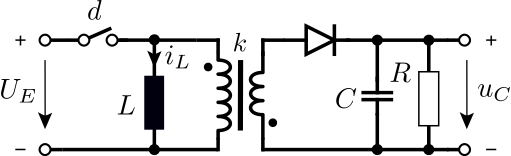
\includegraphics[width=70mm]{Flyback_converter_circuit.pdf}
		\caption{Circuit}
	\end{figure}
	
	%%%%%%%%%%%%%%%%%%%%%% MDOEL EQUATIONS %%%%%%%%%%%%%%%%%%%%%%%%%%%
	
	\section{Model Equations} % MUST
	
	State Vector and Input Vector:
	\begin{align*}
		\underline{x} &= (x_1 \ x_2)^T = (i_L \ u_C)^T \\
		\underline{u} &= d
	\end{align*}
	
	\noindent System Equations:			
	\begin{subequations}
	\begin{align}
		\dot{x}_1 &= -(1-u)\frac{k}{L}x_2 + \frac{U_E}{L}u \\
		\dot{x}_2 &= (1-u)\frac{k}{C}x_1 - \frac{1}{RC}x_2
	\end{align}
	\end{subequations}

	%%%%%%%%%%%%%%%%%%%%%% PARAMETERS | OUTPUTS %%%%%%%%%%%%%%%%%%%%%%%%%%%
	\noindent
	Parameters: $L$ $C$ $R$ $U_E$ $k$ % variables with constant, predefined value
	\\
	Outputs: $x_2 = u_C$
	
	%%%%%%%%%%%%%%%%%%%%%% ASSUMPTIONS %%%%%%%%%%%%%%%%%%%%%%%%%%%
	
	% \subsection{Assumptions} % MAY 
	% 	\begin{enumerate} %possible list type for the Assumptions
	% 		\item The switching frequency is high enough, to prevent the inductor from fully discharging beween charging stages.
	% 	\end{enumerate}
	
	%%%%%%%%%%%%%%%%%%%%%% EXEMPLARY PARAMETER VALUES %%%%%%%%%%%%%%%%%%%%%%%%%%%	
	
	\subsection{Exemplary parameter values}
	\begin{tabular}{cl}
\hline
  Symbol  & Value                                                                                          \\
\hline
   $A$    & $\left[\begin{matrix}0 & 1.0 & 0\\-79.285 & -0.113 & 0\\28.564 & 0.041 & 0\end{matrix}\right]$ \\
   $B$    & $\left[\begin{matrix}0 & 0\\0.041 & -0.0047\\-0.03 & -0.0016\end{matrix}\right]$               \\
 $B_{1}$  & $\left[\begin{matrix}0 & 0\\0.041 & -0.0047\\-0.03 & -0.0016\end{matrix}\right]$               \\
 $C_{1}$  & $\left[\begin{matrix}0 & 0 & 1.0\\1.0 & 0 & 0\\0 & 0 & 0\\0 & 0 & 0\end{matrix}\right]$        \\
   $C$    & $\left[\begin{matrix}0 & 0 & 1.0\\1.0 & 0 & 0\end{matrix}\right]$                              \\
 $D_{11}$ & $\left[\begin{matrix}0\\0\\0\\0\end{matrix}\right]$                                            \\
 $D_{12}$ & $\left[\begin{matrix}0 & 0\\0 & 0\\0.1 & 0\\0 & 0.1\end{matrix}\right]$                        \\
 $D_{21}$ & $\left[\begin{matrix}0\\0\end{matrix}\right]$                                                  \\
\hline
\end{tabular}

	%%%%%%%%%%%%%%%%%%%%%% DERIVATION & EXPLANATION %%%%%%%%%%%%%%%%%%%%%%%%%%%	
	
	\section{Derivation and Explanation} % SHOULD
	See boost converter.
	
	%%%%%%%%%%%%%%%%%%%%%% REFERENCES %%%%%%%%%%%%%%%%%%%%%%%%%%%
	
	\begin{thebibliography}{10}		
		\bibitem{Salimi13}M. Salimi, J. Soltani, A. Zakipour, and V. Hajbani, Sliding mode control of the DC-DC flyback converter with zero steady-state error, in 4th Annual International Power Electronics, Drive Systems and Technologies Conference, Feb. 2013, pp. 158–163. doi: 10.1109/PEDSTC.2013.6506695.
		\bibitem{Roeb17}K. Röbenack, Nichtlineare Regelungssysteme: Theorie und Anwendung der exakten Linearisierung. Berlin, Heidelberg: Springer Berlin Heidelberg, 2017. doi: 10.1007/978-3-662-44091-9.
	\end{thebibliography}

\end{document}

